\subsection{FlashDriver}
	To ensure that in-game high scores are stored despite resets and power outages the values are stored in the AtMega2560's flash memory. To be able to write to the microcontrollers flash memory the following configurations have been made:
	
	\textbf{Page number} \newline
		To store the high score data, we write the top three values in page number 253. The page number is chosen to be a value large enough to ensure that the application code will not overwrite the high score value, while still remaining within the RWW Section of flash memory. This places the first byte of data at address 0xFD00.
	
	\textbf{Flashwriter attribute} \newline
		The FlashWrite function is annotated with \_attribute\_((section (".flashwriter"))). This marks the code for the linker, which then places the code in the \say{.flashwriter} section which is defined in the Linker's MemorySettings under Project Settings, as seen in the figure below.
		
			\begin{figure}[H]
				\centering
				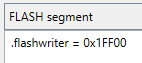
\includegraphics[scale=1.0]{bootloaderAttribute}
				\caption{Address for FlashWrite placement}
				\label{fig:flashwriter}
			\end{figure}
		
		Figure \ref{fig:flashwriter} shows the address section which the FlashWrite method is place. The address 0x1FF00 was chosen due to its placement in the bootloader section. SPM instructions, which are required to do write operations on flash memory, must be executed in the Boot Flash Section. Therefore the address for the bootloader attribute must be within the interval seen in the figure below.
		
			\begin{figure}[H]
				\centering
				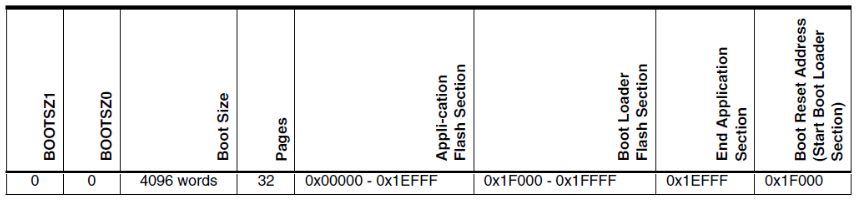
\includegraphics[width=14cm]{bootloaderAddress}
				\caption{Address interval for bootloader}
				\label{fig:bootloaderAddress}
			\end{figure}
	
		The value 0x1FF00 was chosen to avoid being overwritten by the bootloader.

			\begin{figure}[H]
				\centering
				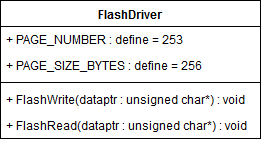
\includegraphics{FlashDriverClassDiagram}
				\caption{Class diagram for FlashDriver}
				\label{fig:FlashDriverClassDiagram}
			\end{figure}	

		Table \ref{tb:methodFlash} describes the methods of FlashDriver.
		
		\begin{table}[H]
			\centering
			\begin{tabular}{|l|l|}
				\hline
				\multicolumn{1}{|c|}{\textbf{Method}} & \multicolumn{1}{c|}{\textbf{Description}} \\ \hline
				FlashWrite & \begin{tabular}[c]{@{}l@{}}This method writes data, which the given pointer is \\pointing to, to three pages in flash memory. Before \\writing to the page, the former contents of the page\\ are erased. \\ This method is executed in the bootloader section of\\ flash memory.\end{tabular} \\ \hline
				FlashRead & \begin{tabular} [c]{@{}l@{}} This method reads data and stores the result in the\\given array.
				\end{tabular} \\ \hline
			\end{tabular}
			\caption{Description of the methods of FlashDriver}
			\label{tb:methodFlash}
		\end{table}